%************************************************
\chapter{Risultati e discussione}\label{ch:risultati}
%************************************************

% ***********************************************
% [ ] Mettere i grafici con le tre classi
% ***********************************************

Qui discuteremo i risultati. 

Per l'implementazione dell'algoritmo è stato scelto il ben noto 
Iris data set. Come evidenziato da Schuld\cite{schuld}, 
l'insieme dati si è dovuto standardizzare e 
normalizzare. Dopo di ciò, il primo passo è stato di 
ripetere l'esperienza dell'articolo per comprenderne 
appieno il funzionamento e poterlo estendere. 
In questo stato, si usano due caratteristiche delle 
quattro disponibili e si possono classificare solo 
due classi alla volta. Inoltre i vettori di apprendimento 
inseriti sono in numero estremamente esiguo e di certo 
insufficiente per garantire una classificazione efficiente. 

%****************************************
% inserire questo discorso nell'introduzione
%*******************************************

Sono state seguite varie linee per migliorare l'algoritmo 
e renderlo più efficace: 
\begin{itemize}
    \item aumentare il numero di classi riconosciute;
    \item aumentare il numero di caratteristiche considerate;
    \item aumentare il numero di vettori di training.
\end{itemize}

%**************************************
% Si possono descrivere i dettagli dell'algoritmo nell'appendice 
%**************************************

Discutiamo con ordine i passi effettuati

Per implementare l'algoritmo si è usato il famoso data set Iris, 
consistente in misure di lunghezze e larghezze di sepali e petali di 
tre varietà di iris. 

\section{Ottimizzazione dei dati}

Inizialmente i dati si presentano nella forma di fig. \ref{fig:iris_grezzi}. 

\begin{figure}[h]
    \centering
    \includegraphics[width=\linewidth]{gfx/iris/iris2features}
    \caption{Dati grezzi}
    \label{fig:iris_grezzi}
\end{figure}

\begin{figure}[h]
    \centering
    \includegraphics[width=\linewidth]{gfx/iris/iris2scaled}
    \caption{Dati standardizzati}
    \label{fig:iris_standard}
\end{figure}

\begin{figure}[h]
    \centering
    \includegraphics[width=\linewidth]{gfx/iris/iris2normalized}
    \caption{Dati normalizzati}
    \label{fig:iris_normal}
\end{figure}

La standardizzazione prevede che si traslino i dati affinché abbiano media nulla, 
dopo di che li scala in modo che abbiano deviazione standard unitaria 
(vedi fig. \ref{fig:iris_standard}). 

A questo punto normalizziamo ciascun vettore (vedi fig. \ref{fig:iris_normal}). 

Avendo effettuato queste operazioni preliminari, si deve ora tradurre le coordinate 
di ciascun vettore nello spazio delle caratteristiche in un angolo di rotazione 
da applicare ad un qubit nella \ac{QRAM}. 

Avendo visto nell'Eq. \ref{eq:qram.prob} che lo stato costruito, dopo la misura condizionale, è 
\begin{equation}
    \sum_{l=0}^{M-1} \psi_{\vec{d}^{(l)}}\ket{\vec{d}^{(l)}}\sin\theta^{(l)}\ket{1}_R,
\end{equation}
troviamo che la relazione esistente tra i valori $b_l$, ovvero le caratteristiche standardizzate e normalizzate, 
e le ampiezze di probabilità nella \ac{QRAM} è 
\begin{equation}
    \theta^{(l)} = \arcsin b_l. 
\end{equation}

\section{Scrittura dell'algoritmo}

Seguendo le istruzioni si costruisce il seguente circuito quantistico. 

%********************************
% la figura del circuito si potrebbe mettere di traverso lungo tutta la pagina
% https://tex.stackexchange.com/a/57531/140965
%********************************

Si noti che questo è espresso usando solo le porte quantistiche presenti 
nell'insieme universale di base messo a disposizione dall'IBM QX. Possiamo infatti notare 
come le porte $C_n R_y (\theta)$ siano in realtà realizzate attraverso una 
successione di più porte. 

Possiamo seguire i passaggi osservando la figura: 
\begin{enumerate}
    \item i qubit ancilla ed indice vengono posti in sovrapposizione uniforme; 
    \item il vettore d'input $x$ è posto in entanglement con lo stato fondamentale 
    dell'ancilla;
    \item il vettore di training $t^0$ è posto in entanglement con lo stato eccitato 
    dell'ancilla e con lo stato fondamentale del qubit indice;
    \item il vettore di training $t^1$ è posto in entanglement con lo stato eccitato 
    dell'ancilla e del qubit indice;
    \item il qubit classe è invertito condizionato dal fatto che il qubit indice sia $\ket{1}$; 
    questo completa la preparazione iniziale dello stato; 
    \item nell'ultimo passaggio la porta Hadamard fa interferire le copie di $x$ con i vettori 
    d'apprendimento e l'ancilla è misurata, seguita da una misura del qubit classe. 
\end{enumerate}
Considereremo validi per i nostri scopi solo le misure del qubit classe ottenute quando il 
qubit ancilla è trovato nello stato $\ket{0}$. 

Si mostra un esempio di risultato di classificazione usando le prime due caratteristiche 
del data set e gli elementi appartenenti alle classi setosa e versicolor. 
Si scelgono come vettori di training un elemento per ciascuna classe, nel nostro caso 
il vettore 34 ed il vettore 86 dal data set, rispettivamente setosa e versicolor. 
Si assegna alla classe setosa lo stato $\ket{0}$ del qubit classe ed alla classe 
versicolor lo stato $\ket{1}$. 
Si sottopongono poi a classificazione, in due esperimenti separati, due vettori sconosciuti: 
il vettore 29 (setosa) ed il vettore 57 (versicolor). 

Il primo passo è simulare l'esperimento sul computer in uso, dato che il problema in esame
è facilmente eseguibile su un comune portatile. I risultati non filtrati per i due esperimenti 
sono visibili in figura. Nella didascalia sono scritti i conteggi corrispondenti ad un 
determinato esito di misura sui due qubit ancilla e classe. La cifra sulla destra contiene la 
misura del qubit ancilla, quella sulla sinistra del qubit classe. Tali valori, normalizzati ad uno, 
sono rappresentati in un istogramma, che approssima la distribuzione di probabilità degli esiti di 
misura per grandi numeri di esecuzioni dell'algoritmo. Per questo motivo si userà preferibilmente 
un numero di esecuzioni pari al massimo permesso sui computer quantistici dell'IBM, ovvero 8192. 

\begin{figure}[h]
    \myfloatalign
    \subfloat[Iris setosa] {
        \label{fig:misura_setosa}
        \includegraphics[width=\linewidth]{gfx/misura_setosa}
    } \\
    \subfloat[Iris versicolor] {
        \label{fig:misura_versicolor}
        \includegraphics[width=\linewidth]{gfx/misura_versicolor}
    }
    \caption{Simulazione del circuito. I conteggi totali sono\\
    per setosa: \{'00': 3843, '10': 2056, '01': 352, '11': 1941\}; \\
    per versicolor: \{'00': 2749, '10': 3908, '01': 1414, '11': 121\}.}
    \label{fig:simulazione_circuito}
\end{figure}

Selezionando i risultati laddove il bit di destra è 0, abbiamo praticamente effettuato 
la misura condizionale necessaria al funzionamento dell'algoritmo. 

\begin{figure}[h]
    \myfloatalign
    \subfloat[Iris setosa]{
        \label{fig:misura_setosa_filtrata}
        \includegraphics[width=\linewidth]{gfx/misura_setosa_filtrata}
    } \\
    \subfloat[Iris versicolor]{
        \label{fig:misura_versicolor_filtrata}
        \includegraphics[width=\linewidth]{gfx/misura_versicolor_filtrata}
    }
    \caption{Simulazione del circuito, risultati filtrati}
    \label{fig:simulazione_filtrati}
\end{figure}

Il passo successivo è eseguire questi stessi circuiti quantistici su un vero computer quantistico. 
È usata scelta la macchina a 14 qubit ibmq\_16\_melbourne per ottenere le seguenti misure per il vettore d'input 
setosa. 

\begin{figure}[h]
    \centering
    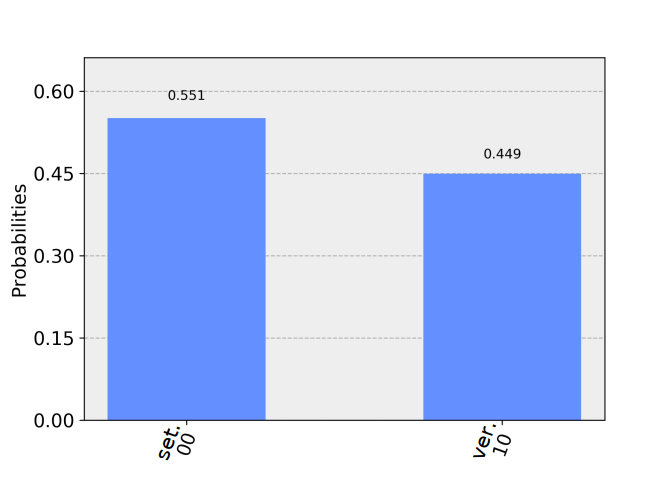
\includegraphics[width=\linewidth]{gfx/misura_setosa_sperimentale}
    \caption{Esecuzione su hardware reale (setosa)}
    \label{fig:sperimentale_setosa}
\end{figure}

Gli inevitabili fenomeni di rumore rendono i risultati meno piccati ma comunque 
distinguibili in questo caso. 

Si noti che fino ad ora non è stato fatto uso delle tecniche di costruzione \ac{QRAM} 
introdotte nella sezione \ref{sec:ff-qram}. 

L'obiettivo principale di questa tesi è cercare di ottenere un algoritmo multiclasse generico 
a partire da quello appena discusso. Si può dire che le seguenti sottosezioni segnano il vero e proprio 
punto di inizio del lavoro originale in questa tesi\footnote{È possibile trovare lavori analoghi 
a questo in rete, si veda a titolo di esempio gli algoritmi sviluppati da Carsten Blank su 
\url{https://github.com/carstenblank/dc-qiskit-qml}}. 

Sebbene si potrebbe mirare subito ad aumentare il numero di classi riconosciute, dobbiamo tenere 
conto di un problema che si deve affrontare quando si ha a che fare con data set simili ad Iris: 
le classi versicolor e virginica non sono ben distinguibili; infatti se avessimo effettuato una 
misura considerando solo due feature, come abbiamo appena fatto, avremmo ottenuto risultati vaghi 
(probabilità intorno al 50\% per entrambi i risultati) o addirittura erronei. 

Un modo di aggirare il problema consiste nell'uso di feature map\cite{schuld}, ovvero funzioni polinomiali che, 
applicate al data set, ci restituiscono una nuova configurazione dei vettori di apprendimento da 
usare per il training e per la classificazione. Usando una feature map appropriata, si possono 
separare in maniera sufficiente vettori appartenenti a classi diverse e migliorare l'efficienza 
del riconoscimento. 

Questa tesi non adotta tale tecnica, in quanto il suo scopo è verificare come scala in grandezza 
l'algoritmo \ac{KNN} quantistico appena illustrato. Si tenta dunque di migliorare l'efficienza 
del riconoscimento aumentando il numero di caratteristiche, dunque la dimensionalità, dell'insieme 
dei vettori di training. 

\subsection{Aumento delle numero di caratteristiche}

\marginpar{La maggior parte dei vettori versicolor 
e virginica non vengono classificati correttamente, qui abbiamo selezionato un caso in cui la 
classificazione è corretta fin dal caso più semplice.}
Per verificare il miglioramento apportato da un aumento del numero di caratteristiche 
considerate, si prende in esame la classificazione del vettore d'input 54 (versicolor), 
con i vettori di training numero 51 (versicolor) e 146 (virginica) del data set. 
Il vettore d'input viene classificato correttamente durante la simulazione 
con probabilità vicina al 51.4\%. 
Effettuando la stessa misura, ma tenendo conto di tutte le quattro feature, arriviamo ad 
una probabilità di classificazione corretta del 58.3\% nel migliore dei casi. Questo è un 
segno che l'implementazione ha un margine di miglioramento apprezzabile. 

\subsection{Aumento del numero di vettori d'apprendimento}

Per poter implementare più di due classi, è necessario essere capaci di 
memorizzare almeno tre vettori di apprendimento, per poi associare ad ognuno di essi la 
rispettiva classe. 
L'aggiunta di vettori di training, riprendendo in esame il confronto tra classi 
versicolor e virginica, non ha effetti ben prevedibili, almeno per piccoli 
insiemi. Aggiungendo altri due vettori d'apprendimento si possono migliorare o 
peggiorare i risultati, a seconda della disposizione dei vettori nello spazio delle 
caratteristiche; si rende necessario un criterio di selezione dei vettori più 
significativi per ottenere un classificatore il più efficace possibile, 
non potendo inserire tutti i vettori del data set, 
e tantomeno potendo scegliere a caso i vettori finché non si 
riscontra il risultato aspettato (il presupposto di un algoritmo maturo è che 
una volta ultimato non debba aver bisogno di aggiustamenti significativi da 
parte dell'operatore umano). Oltretutto una scelta manuale degli specifici vettori 
di training potrebbe andare bene per i vettori d'input su cui si sta concentrando 
in un dato momento, ma non si può conoscere l'efficacia rispetto a eventuali 
nuovi vettori sconosciuti. 

\subsection{Implementazione multiclasse}

L'aggiunta della capacità di riconoscere tutte le tre classi in una sola esecuzione 
non è di natura differente dall'aggiungere qubit per avere maggiori vettori 
di addestramento. Passiamo dall'avere un solo qubit classe, che ha associato il 
proprio stato  
$\ket{0}$ alla prima classe e lo stato $\ket{1}$ alla seconda, ad avere due qubit 
ed associare lo stato $\ket{00}$ alla prima classe, lo stato $\ket{01}$ alla 
seconda classe e lo stato $\ket{10}$ alla terza classe. Lo stato $\ket{11}$ resta 
inutilizzato. 

Nel processo di costruzione della \ac{QRAM} contenente lo stato iniziale, 
oltre che ai qubit indice, i vettori di addestramento saranno in entanglement 
anche con i due qubit classe, nella maniera appropriata per ogni vettore. 

\section{Esecuzione completa}

Per studiare l'efficienza dell'algoritmo a diversi stadi di miglioramento, 
si divide il data set in un insieme dedicato all'addestramento ed un insieme 
di vettori da classificare. Al fine di avere risultati statisticamente 
rilevanti, per ogni esecuzione i vettori di training ed il vettore d'input 
sono scelti casualmente a partire dal data set completo. 
Si contano le classificazioni di successo 
rispetto al totale dei tentativi, al variare dei parametri come il numero 
di features o il numero di vettori di training usati. 

Provando ad effettuare una classificazione a tre classi con 32 vettori di 
training otteniamo i seguenti esiti: 
\begin{itemize}
    \item i vettori della classe setosa sono correttamente classificati 10 volte su 10;
    \item i vettori della classe versicolor sono correttamente classificati 5 volte su 10;
    \item i vettori della classe virginica sono correttamente clasificati 9 volte su 10.
\end{itemize}
I risultati vengono necessariamente da simulazioni, in quanto sono necessari 
19 qubit sotto queste condizioni. 
